\documentclass{article}

% Language setting
% Replace `english' with e.g. `spanish' to change the document language
\usepackage[spanish]{babel}

% Set page size and margins
% Replace `letterpaper' with `a4paper' for UK/EU standard size
\usepackage[letterpaper,top=2cm,bottom=2cm,left=3cm,right=3cm,marginparwidth=1.75cm]{geometry}

% Useful packages
\usepackage{amsmath}
\usepackage{graphicx}
\usepackage{enumitem}
\usepackage{comment}
\usepackage{wrapfig}
\usepackage{amssymb}
\usepackage[colorlinks=true, allcolors=blue]{hyperref}
\usepackage{tikz}
\usepackage{etoolbox}
\usetikzlibrary{matrix,positioning,chains,fit,shapes,calc}
\definecolor{myblue}{RGB}{80,80,160}
\definecolor{mygreen}{RGB}{80,160,80}

\title{Matemática Discreta Tema 4. Grafos}
\author{Martín González Dios 
\href{https://github.com/martindios}{\includegraphics[height=0.5cm]{github.png}}}

\begin{document}
\maketitle

Un grafo \textbf{G = (V, E)} consistente en V, un conjunto no vacío de vértices o nodos y E, un conjunto de aristas. \\

\section{Tipos de grafos}

\subsection{Grafo Simple}
Es un grafo que no tiene bucles (aristas que conectan un vértice consigo mismo) ni aristas múltiples (dos o más aristas que conectan el mismo par de vértices). En un grafo simple, cada par de vértices está conectado por a lo sumo una arista.

\begin{figure}[h]
    \centering
    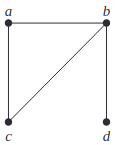
\includegraphics[width=0.14\textwidth]{img-t4/img_912_48.png}
    \caption{Grafo simple}
\end{figure}

\subsection{Mutligrafo}
Es un tipo de grafo que \textbf{permite múltiples aristas entre el mismo par de vértices}. Es decir, puede haber dos o más aristas que conecten los mismos vértices. (Existen varios caminos para ir de un nodo a otro)

\begin{figure}[h]
    \centering
    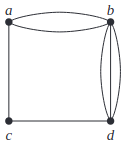
\includegraphics[width=0.14\textwidth]{img-t4/img_205_31.png}
    \caption{Multigrafo}
\end{figure}

\newpage

\subsection{Grafo ponderado}
Es un grafo en el que \textbf{cada arista tiene un peso o costo asociado}. Este peso puede representar distancias, costos, tiempos, etc.

\begin{figure}[h]
    \centering
    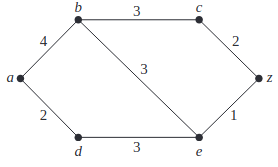
\includegraphics[width=0.34\textwidth]{img-t4/img_168_10.png}
    \caption{Grafo ponderado}
\end{figure}

\subsection{Grafo dirigido}
En un grafo dirigido, \textbf{las aristas tienen una dirección}, lo que significa que van de un vértice a otro y no se puede recorrer en sentido contrario. 

\begin{figure}[h]
    \centering
    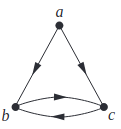
\includegraphics[width=0.14\textwidth]{img-t4/img_131_39.png}
    \caption{Grafo dirigido}
\end{figure}

\subsection{Grafo completo}
Es un grafo simple que cada par de vértices están conectados por una arista. El número de aristas del grafo completo $K_n$ es: 
$$|E| = \frac{n(n-1)}{2}$$

    \begin{center}
    \begin{tikzpicture}
    % Definimos los vértices
    \foreach \i in {1,2,3,4,5} {
        \pgfmathsetmacro{\angle}{360/5 * \i - 90} % Ángulo para la posición de los vértices
        \node[circle, draw, fill=white, minimum size=0.5cm] (v\i) at (\angle:1.5) {};
    }

    % Dibujamos las aristas
    \foreach \i in {1,2,3,4,5} {
        \foreach \j in {1,2,3,4,5} {
            \ifnum\i<\j
                \draw[thick] (v\i) -- (v\j);
            \fi
        }
    }
    \end{tikzpicture}
    $K_5$
    \end{center}

\newpage

\section{Grado de un vértice}
El grado de un vértice en un grafo es una medida que indica \textbf{cuántas aristas están conectadas a ese vértice}. Se denomina como $\delta(vertice)$ = grado.
Dependiendo del tipo de grafo, el grado se puede definir de la siguiente manera:

\begin{itemize}
    \item Grafo no dirigido: en un grafo no dirigido, el grado de un vértice es simplemente el número de aristas que inciden en él. Por ejemplo, si un vértice tiene tres aristas conectadas, su grado es 3.

    \item Grafo dirigido: En un grafo dirigido, se distingue entre dos tipos de grado:
        1. \textbf{Grado de entrada}: es el número de aristas que llegan al vértice (es decir, que apuntan hacia él).
        2. \textbf{Grado de salida}: es el número de aristas que salen del vértice (es decir, que apuntan desde él).
        3. El \textbf{grado total} de un vértice en un grafo dirigido se puede considerar como la suma del grado de entrada y el grado de salida.
\end{itemize}

Dado un grafo G = (V, E), siendo V los vértices y E las aristas: 
$$\sum_{v \in V} \delta(v) = 2 \cdot |E|$$

\section{Representación de un grafo}

Los grafos se pueden representar mediante una matriz de adyacencia. A continuación, se presenta un ejemplo.

\subsection*{Ejemplo}

Consideremos un grafo con los siguientes vértices y aristas:

\begin{itemize}
    \item Vértices: $ A, B, C, D $
    \item Aristas: $ (A, B), (A, C), (B, D) $
\end{itemize}

La matriz de adyacencia para este grafo es:

$$\begin{array}{c|cccc}   & A & B & C & D \\ \hline A & 0 & 1 & 1 & 0 \\ B & 1 & 0 & 0 & 1 \\ C & 1 & 0 & 0 & 0 \\ D & 0 & 1 & 0 & 0 \\ \end{array}$$

$$
\begin{bmatrix}
0 & 1 & 1 & 0 \\
1 & 0 & 0 & 1 \\
1 & 0 & 0 & 0 \\
0 & 1 & 0 & 0
\end{bmatrix}
$$

\begin{center}
\begin{tikzpicture}[scale=1]
    % Definición de los nodos
    \node[circle, draw] (A) at (0, 1) {A};
    \node[circle, draw] (B) at (1, 2) {B};
    \node[circle, draw] (C) at (1, 0) {C};
    \node[circle, draw] (D) at (2, 1) {D};

    % Definición de las aristas
    \draw (A) -- (B);
    \draw (A) -- (C);
    \draw (B) -- (D);
    \draw (C) -- (A);
    \draw (D) -- (B);
\end{tikzpicture}
\end{center}

\section{Subgrafo}

\begin{center}
\begin{tikzpicture}[scale=1]
    % Definición de los nodos
    \node[circle, draw] (A) at (0, 1) {A};
    \node[circle, draw] (B) at (1, 2) {B};
    \node[circle, draw] (C) at (1, 0) {C};
    \node[circle, draw] (D) at (2, 1) {D};

    % Definición de las aristas
    \draw (A) -- (B);
    \draw (A) -- (C);
    \draw (B) -- (D);
    \draw (C) -- (A);
    \draw (D) -- (B);
\end{tikzpicture}
(Grafo de referencia para ejemplos en subgrafos)
\end{center}

Un \textbf{subgrafo} $ H $ de un grafo $ G = (V, E) $ es un grafo que se forma a partir de un subconjunto de los vértices $ V' \subseteq V $ y un subconjunto de las aristas $ E' \subseteq E $ tales que cada arista en $ E' $ conecta dos vértices en $ V' $. Formalmente, se puede definir como:

$$H = (V', E') \quad \text{donde} \quad V' \subseteq V \quad \text{y} \quad E' \subseteq E \text{ y } E' \text{ contiene solo aristas entre vértices en } V'.$$

\begin{center}
\begin{tikzpicture}[scale=1]
    % Definición de los nodos
    \node[circle, draw] (A) at (0, 1) {A};
    \node[circle, draw] (B) at (1, 2) {B};
    \node[circle, draw] (C) at (1, 0) {C};

    % Definición de las aristas
    \draw (A) -- (B);
    \draw (A) -- (C);
\end{tikzpicture}
\end{center}

\subsection{Subgrafo propio}
Un \textbf{subgrafo propio} de un grafo $ G $ es un subgrafo $ H $ que no es igual a $ G $ en términos de sus vértices y aristas. Es decir, $ H $ es un subgrafo propio de $ G $ si:

$$H \neq G.$$

Esto implica que $ V' $ es un subconjunto propio de $ V $ (es decir, $ V' \neq V $) o $ E' $ es un subconjunto propio de $ E $ (es decir, $ E' \neq E $).

\begin{center}
\begin{tikzpicture}[scale=1]
    % Definición de los nodos
    \node[circle, draw] (B) at (1, 2) {B};
    \node[circle, draw] (D) at (2, 1) {D};

    % Definición de las aristas
    \draw (B) -- (D);
\end{tikzpicture}
\end{center}

\subsection{Subgrafo generador}

Un \textbf{subgrafo generador} de un grafo $ G $ es un subgrafo que contiene todos los vértices de $ G $ pero puede tener un subconjunto de las aristas. En otras palabras, un subgrafo generador $ H $ de $ G $ es tal que:

$$V' = V \quad \text{y} \quad E' \subseteq E.$$

Esto significa que $ H $ incluye todos los vértices de $ G $ y puede incluir algunas o todas las aristas de $ G $.

\begin{center}
\begin{tikzpicture}[scale=1]
    % Definición de los nodos
    \node[circle, draw] (A) at (0, 1) {A};
    \node[circle, draw] (B) at (1, 2) {B};
    \node[circle, draw] (C) at (1, 0) {C};
    \node[circle, draw] (D) at (2, 1) {D};

    % Definición de las aristas
    \draw (A) -- (B);
    \draw (A) -- (C);
\end{tikzpicture}
\end{center}

\section{Formar de recorrer un grafo}
Un \textbf{camino} es una secuencia de vértices en un grafo donde cada par de vértices consecutivos está conectado por una arista. Formalmente, un camino se puede definir como una secuencia de vértices $ v_1, v_2, \ldots, v_k $ tal que existe una arista entre $ v_i $ y $ v_{i+1} $ para $ i = 1, 2, \ldots, k-1 $. \\

Tipos de camino:
\begin{enumerate}
    \item \textbf{Camino Simple:} un camino es simple si no repite ningún vértice. Es decir, todos los vértices en el camino son distintos.

    \item \textbf{Camino Cerrado:} un camino es cerrado si el primer y el último vértice son el mismo. En otras palabras, forma un ciclo.

    \item \textbf{Camino Abierto:} un camino es abierto si el primer y el último vértice son diferentes. Este es el tipo más común de camino.
\end{enumerate}

\section{Isomorfismo de grafos}
Dos grafos $ G = (V_G, E_G) $ y $ H = (V_H, E_H) $ se dicen \textbf{isomorfos} si existe una biyección $ f: V_G \to V_H $ tal que para cualesquiera dos vértices $ u, v \in V_G $, se cumple que:

$$\{u, v\} \in E_G \iff \{f(u), f(v)\} \in E_H.$$

Esto significa que hay una correspondencia uno a uno entre los vértices de los dos grafos que preserva la estructura de las aristas. \\

La manera de \textbf{comprobar si dos grafos son isomorfos} es ir comparándolos vértice a vértice y comprobar que cada vértice se conecta con el correspondiente en el otro grafo, además de comprobar que el grado de los grafos sea el mismo.

\subsection{Propiedades del Isomorfismo}

\begin{enumerate}
    \item \textbf{Preservación de la Conectividad}: si dos grafos son isomorfos, tienen la misma conectividad. Es decir, si hay un camino entre dos vértices en un grafo, habrá un camino correspondiente entre los vértices isomorfos en el otro grafo.

    \item \textbf{Número de Vértices y Aristas}: dos grafos isomorfos deben tener el \textbf{mismo número de vértices y el mismo número de aristas}.

    \item \textbf{Grados de los Vértices}: si $ G $ y $ H $ son isomorfos, entonces para cada vértice $ v $ en $ G $, el grado de $ v $ (número de aristas incidentes) debe ser igual al grado del vértice correspondiente $ f(v) $ en $ H $.

    \item \textbf{Ciclos y Componentes Conexas}: los ciclos y componentes conexas en un grafo se preservan en su grafo isomorfo.
\end{enumerate}

\subsection{Ejemplo de Isomorfismo}

\begin{tikzpicture}[Bullet/.style={circle,draw,fill=black,inner sep=1.5pt},
adjacency matrix/.style={ampersand replacement=\&,matrix of math nodes,
 row 1/.append style={nodes={font=\boldmath}},
 column 1/.append style={nodes={font=\boldmath}},nodes in empty cells,
nodes={draw,minimum width=1.5em,text height=1.8ex},column sep=-\pgflinewidth,row
sep=-\pgflinewidth}]
% first matrix
\def\adjancymatrix{%
{{0,0,1,1,0},%
{0,0,0,1,1},%
{1,0,0,0,1},%
{1,1,0,0,0},%
{0,1,1,0,0}}} 
 \let\mymatrixcontent\empty
 \def\mymatrixcontent{|[draw=none]|\& 1 \& 2 \& 3 \& 4  \& 5\\}
 \begin{scope}[local bounding box=left]
  \foreach \X in {1,...,5}
   {\node[Bullet,label=90+72-\X*72:{$e_\X$}] (E\X) at (90+72-\X*72:2) {} ;}
  \foreach \X in {1,...,5}
  {\begingroup\edef\x{\endgroup
         \noexpand\gappto\noexpand\mymatrixcontent{\X }}\x
  \foreach \Y in {1,...,5}
   {\pgfmathtruncatemacro{\itest}{\adjancymatrix[\X-1][\Y-1]}
   \ifnum\itest=1
    \draw (E\X) -- (E\Y);
    \begingroup\edef\x{\endgroup
         \noexpand\gappto\noexpand\mymatrixcontent{\& 1 }}\x
   \else
    \begingroup\edef\x{\endgroup
         \noexpand\gappto\noexpand\mymatrixcontent{ \&}}\x
   \fi
   }
   \gappto\mymatrixcontent{\\}
   }
 \end{scope} 
 \matrix (leftmat) [below=of left,adjacency matrix]{
    \mymatrixcontent
  };
 %
% second matrix
\def\adjancymatrix{%
{{0,1,0,0,1},%
{1,0,1,0,0},%
{0,1,0,1,0},%
{0,0,1,0,1},%
{1,0,0,1,0}}} 
 \let\mymatrixcontent\empty
 \def\mymatrixcontent{|[draw=none]|\& 1 \& 2 \& 3 \& 4  \& 5\\}
 \begin{scope}[local bounding box=middle,xshift=5cm]
  \foreach \X in {1,...,5}
   {\node[Bullet,label=90+72-\X*72:{$e_\X$}] (E\X) at (90+72-\X*72:2) {} ;}
  \foreach \X in {1,...,5}
  {\begingroup\edef\x{\endgroup
         \noexpand\gappto\noexpand\mymatrixcontent{\X }}\x
  \foreach \Y in {1,...,5}
   {\pgfmathtruncatemacro{\itest}{\adjancymatrix[\X-1][\Y-1]}
   \ifnum\itest=1
    \draw (E\X) -- (E\Y);
    \begingroup\edef\x{\endgroup
         \noexpand\gappto\noexpand\mymatrixcontent{\& 1 }}\x
   \else
    \begingroup\edef\x{\endgroup
         \noexpand\gappto\noexpand\mymatrixcontent{ \&}}\x
   \fi
   }
   \gappto\mymatrixcontent{\\}
   }
 \end{scope} 
 \matrix (midmat) [below=of middle,adjacency matrix]{
    \mymatrixcontent
  };
% third matrix
\def\adjancymatrix{%
{{0,1,0,1,0},%
{1,0,0,0,1},%
{0,0,0,1,1},%
{1,0,1,0,0},%
{0,1,1,0,0}}} 
 \let\mymatrixcontent\empty
 \def\mymatrixcontent{|[draw=none]|\& 1 \& 2 \& 3 \& 4  \& 5\\}
 \begin{scope}[local bounding box=right,xshift=10cm]
  \foreach \X in {1,...,3}
   {\node[Bullet,label=90+72-\X*72:{$e_\X$}] (E\X) at (90+72-\X*72:2) {} ;}
  \node[Bullet,label=90+72-4*72:{$e_5$}] (E5) at (90+72-4*72:2) {} ; 
  \node[Bullet,label=90+72-5*72:{$e_4$}] (E4) at (90+72-5*72:2) {} ; 
  \foreach \X in {1,...,5}
  {\begingroup\edef\x{\endgroup
         \noexpand\gappto\noexpand\mymatrixcontent{\X }}\x
  \foreach \Y in {1,...,5}
   {\pgfmathtruncatemacro{\itest}{\adjancymatrix[\X-1][\Y-1]}
   \ifnum\itest=1
    \draw (E\X) -- (E\Y);
    \begingroup\edef\x{\endgroup
         \noexpand\gappto\noexpand\mymatrixcontent{\& 1 }}\x
   \else
    \begingroup\edef\x{\endgroup
         \noexpand\gappto\noexpand\mymatrixcontent{ \&}}\x
   \fi
   }
   \gappto\mymatrixcontent{\\}
   }
 \end{scope} 
 \matrix (rightmat) [below=of right,adjacency matrix]{
    \mymatrixcontent
  };

\end{tikzpicture}

\section{Matriz de incidencia}
La \textbf{matriz de incidencia} es una representación matricial de un grafo que relaciona sus vértices con sus aristas. Para un grafo $ G $ con $ n $ vértices y $ m $ aristas, la matriz de incidencia $ M $ es una matriz de tamaño $ n \times m $ donde:

$$M[i,j] = \begin{cases} 1 & \text{si el vértice } i \text{ está adyacente con la arista } j, \\ 0 & \text{en caso contrario.} \end{cases}$$

\newpage

\subsection{Ejemplo de Matriz de Incidencia}

Consideremos el siguiente grafo $ G $:

\begin{center}
\begin{tikzpicture}[scale=1]
    \node[circle, draw] (v1) at (0, 1) {v1};
    \node[circle, draw] (v2) at (1, 2) {v2};
    \node[circle, draw] (v3) at (3, 2) {v3};
    \node[circle, draw] (v4) at (3, 0) {v4};
    \node[circle, draw] (v5) at (2, -1) {v5};
    \node[circle, draw] (v6) at (1, -2) {v6};
    \node[circle, draw] (v7) at (0, -1) {v7};


    \draw (v1) -- (v2) node[midway, above] {e1};
    \draw (v2) -- (v3) node[midway, above] {e2};
    \draw (v3) -- (v4) node[midway, above] {e3};
    \draw (v4) -- (v5) node[midway, above] {e4};
    \draw (v5) -- (v6) node[midway, above] {e5};
    \draw (v6) -- (v7) node[midway, above] {e6};
    \draw (v3) -- (v7) node[pos=0.7, above right] {e7};
    \draw (v2) -- (v5) node[pos=0.3, above left] {e8};
\end{tikzpicture}
\end{center}


$$M = \begin{bmatrix} 
1 & 0 & 0 & 0 & 0 & 0 & 0 & 0 \\
1 & 1 & 0 & 0 & 0 & 0 & 0 & 1 \\
0 & 1 & 1 & 0 & 0 & 0 & 1 & 0 \\
0 & 0 & 1 & 1 & 0 & 0 & 0 & 0 \\
0 & 0 & 0 & 1 & 1 & 0 & 0 & 1 \\
0 & 0 & 0 & 0 & 1 & 1 & 0 & 0 \\
0 & 0 & 0 & 0 & 0 & 1 & 1 & 0 \\
\end{bmatrix}$$

Siendo las columnas las aristas de $e1$ a $e8$ y las filas los vértices de $v1$ a $v7$.

\section{Conectividad de un grafo}
El número de caminos de longitud $k$ que hay entre un vértice $v_i$ y el vértice $v_j$ es la entrada (i, j) de la matriz de adyacencia $A^k$. \\

\textbf{Ejemplo}: ¿Caminos de longitud 3 entre $v4$ y $v1$ del siguiente grafo?

\begin{center}
\begin{tikzpicture}[scale=1]
    \node[circle, draw] (v1) at (-1, 1.5) {v1};
    \node[circle, draw] (v2) at (1, 2) {v2};
    \node[circle, draw] (v3) at (2, 0) {v3};
    \node[circle, draw] (v4) at (0, 0) {v4};

    \draw (v1) -- (v4) node[midway, above];
    \draw (v2) -- (v4) node[midway, above];
    \draw (v3) -- (v4) node[midway, above];
    \draw (v2) -- (v3) node[midway, above];
    \draw (v3) edge[loop above] (v3);
    \draw (v2) edge[loop above] (v2);

\end{tikzpicture}
\end{center}

$$A = \begin{bmatrix} 
0 & 0 & 0 & 1 \\
0 & 1 & 1 & 1 \\
0 & 1 & 1 & 1 \\
1 & 1 & 1 & 0 \\
\end{bmatrix}$$

$$A^3 = \begin{bmatrix} 
0 & 2 & 2 & 3 \\
2 & 8 & 8 & 7 \\
2 & 8 & 8 & 7 \\
3 & 7 & 7 & 4 \\
\end{bmatrix}$$

$A^3$(4, 1) = 3. \textbf{Existen 3 caminos posibles}.

\section{Grafo bipartito}
Se considera grafo bipartito si tiene una partición de dos conjuntos de vértices, $V_1$ y $V_2$. Cada conjunto está unido vértice a vértice por una arista.

\begin{tikzpicture}[thick,
  fsnode/.style={},
  ssnode/.style={},
  every fit/.style={ellipse,draw,inner sep=5pt,text width=2cm},
  ->,shorten >= 3pt,shorten <= 3pt
]

% the vertices of U
\begin{scope}[start chain=going below,node distance=7mm]
\foreach \i/\xcoord/\ycoord in {1/6/8,2/5/1,3/-4/7,4/6/9,5/0/-3}
  \node[fsnode,on chain,label=left:$t_{\i}$] (f\i) {$(\xcoord,\ycoord)$};
\end{scope}

% the vertices of V
\begin{scope}[xshift=4cm,yshift=-0.5cm,start chain=going below,node distance=7mm]
\foreach \i/\xcoord/\ycoord in {6/0/3,7/1/4,8/-2/1,9/5/9}
  \node[ssnode,on chain,label=right:$t_{\i}$] (s\i) {$(\xcoord,\ycoord)$};
\end{scope}

% the set U
\node [myblue,fit=(f1) (f5),label=above:$U$] {};
% the set V
\node [mygreen,fit=(s6) (s9),label=above:$V$] {};

% the edges
\draw (f1) -- (s6);
\draw (s6) -- (f2);
\draw (f2) -- (s7);
\draw (s7) -- (f3);
\draw (s8) -- (f3);
\draw (f3) -- (s9);
\draw (s9) -- (f5);
\draw (f5) -- (s6);
\end{tikzpicture}
Ejemplo de grafo bipartito.

\subsection{Características de los grafos bipartitos}
Grafo bipartito G = $(V_1 \cup V_2, E)$, con $V_1 = \{v_1, ..., v_n\}$ y $V_2 = \{w_1, ..., w_n\}$

$$\sum_{i=1}^n gr(v_i) + \sum_{i=1}^m gr(w_i) = |E|$$
\textbf{La suma de los grados de los 2 conjuntos da el total de las aristas}. \\

Un grafo G es \textbf{bipartito si G no tiene ciclos de longitud impar}. \\

Para determinar si un grafo es bipartito basta con ir coloreando los vértices, cuando sean adyacentes se cambia de color.

\newpage

\subsection{Grafo bipartito completo}
Si cada uno de los vértices de un subconjunto de la partición es \textbf{vecino de todos los vértices del otro subconjunto}. El grafo bipartito completo se designa como $K_{n, m}$. \\
G($V_1 \cup V_2$, E). $|V_1|$ = n, $|V_2|$ = m. \\

\textbf{Propiedades} del grafo bipartito: \\ 
$$|E| = n \cdot m$$
Todo grafo bipartito es isomorfo a un subgrafo de un grafo completo $K_{n, m}$.


\tikzset{unode/.style = {
    circle, 
    draw=cyan!30!black, 
    thick,
    fill=cyan!80!black,
    inner sep=2.3pt,
    minimum size=2.3pt } }
\tikzset{uedge/.style = {
    draw=cyan!20!black, 
    very thick} }

\begin{center}
\begin{tikzpicture}[scale=2.1] 
    \begin{scope}
        \newcommand\m{4}    
        \newcommand\n{5}    % bottom row, should be weakly larger than m

        \foreach \i in {1,...,\m}{
            \node[unode] (t\i) at (-0.5*\m + \i,1) {};
        }
        \foreach \j in {1,...,\n} {
            \node[unode] (b\j) at (-0.5*\n + \j,0) {};
            \foreach \i in {1,...,\m}{
                \path[uedge] (b\j) edge (t\i);
            }
        }
        \node at (0.5,-0.3) {$K_{\m,\n}$};
    \end{scope}

    \begin{scope}[yshift=2cm]
        \newcommand\m{3}    
        \newcommand\n{6}    % bottom row, should be weakly larger than m

        \foreach \i in {1,...,\m}{
            \node[unode] (t\i) at (-0.5*\m + \i,1) {};
        }
        \foreach \j in {1,...,\n} {
            \node[unode] (b\j) at (-0.5*\n + \j,0) {};
            \foreach \i in {1,...,\m}{
                \path[uedge] (b\j) edge (t\i);
            }
        }
        \node at (0.5,-0.3) {$K_{\m,\n}$};
    \end{scope}
\end{tikzpicture}
\end{center}

\section{Grafo plano}
Un grafo es plano si se puede dibujar en el plano sin que \textbf{ninguna de sus aristas se cruce}.

\subsection{Propiedades}
\begin{enumerate}
    \item Sea un grafo \textbf{conexo, sin bucles y plano} G = (V, E), con $|V| \geq 3$, \textbf{entonces} $|E| \leq 3 |V| - 6$.
    $K_5$ no es plano ($10 \leq 3 \cdot 5 - 6$)

    \begin{center}
    \begin{tikzpicture}
    % Definimos los vértices
    \foreach \i in {1,2,3,4,5} {
        \pgfmathsetmacro{\angle}{360/5 * \i - 90} % Ángulo para la posición de los vértices
        \node[circle, draw, fill=white, minimum size=0.5cm] (v\i) at (\angle:1.5) {};
    }

    % Dibujamos las aristas
    \foreach \i in {1,2,3,4,5} {
        \foreach \j in {1,2,3,4,5} {
            \ifnum\i<\j
                \draw[thick] (v\i) -- (v\j);
            \fi
        }
    }
    \end{tikzpicture}
    $K_5$
    \end{center}

    \item Sea un grafo \textbf{conexo, bipartito y plano} G = (V, E) con $|V| \geq 3$, \textbf{entonces}  $|E| \leq 2 |V| - 4$. \\
    $K_{3, 3}$ no es plano ($9 \nleqslant 2 \cdot 6 - 4$)

    \begin{center}
    \begin{tikzpicture}[scale=1]
    \node[circle, draw] (v1) at (0, 2) {v1};
    \node[circle, draw] (v2) at (0, 0) {v2};
    \node[circle, draw] (v3) at (2, 0) {v3};
    \node[circle, draw] (v4) at (2, 2) {v4};
    \node[circle, draw] (v5) at (4, 2) {v5};
    \node[circle, draw] (v6) at (4, 0) {v6};

    \draw (v1) -- (v2) node[midway, above];
    \draw (v3) -- (v4) node[midway, above];
    \draw (v5) -- (v6) node[midway, above];
    \draw (v1) -- (v3) node[midway, above];
    \draw (v1) -- (v6) node[midway, above];
    \draw (v5) -- (v2) node[midway, above];
    \draw (v5) -- (v3) node[midway, above];
    \draw (v4) -- (v2) node[midway, above];
    \draw (v4) -- (v6) node[midway, above];

\end{tikzpicture}
$K_{3, 3}$
\end{center}
    
\end{enumerate}

\section{Teorema de Kuratowski}
El Teorema de Kuratowski establece que un grafo es plano si, y solo si, no contiene ningún subgrafo que sea homeomorfo a $ K_5 $ o $ K_{3, 3} $. 

\subsection{Definiciones}

\begin{itemize}
    \item Un \textbf{grafo plano} es aquel que puede ser dibujado en el plano sin que sus aristas se crucen.
    \item Dos grafos son \textbf{homeomorfos} si se pueden obtener uno del otro mediante sucesivas subdivisiones de sus aristas. Esto significa que se pueden agregar vértices en las aristas sin cambiar la estructura fundamental del grafo.
    \item $ K_5 $ es el grafo completo de cinco vértices, donde cada par de vértices está conectado por una arista.
    \item $ K_{3, 3} $ es un grafo bipartito completo que tiene dos conjuntos de tres vértices, donde cada vértice de un conjunto está conectado a todos los vértices del otro conjunto.
\end{itemize}

\newpage

\subsection{Ejemplo}

\begin{center}
\begin{tikzpicture}
  \tikzstyle{vertex}=[circle,draw=black,fill=black!20,minimum size=18pt,inner sep=0pt]
  \draw (0,0) node (c){};

  \draw (c)++(0*360/4+135:3) node[vertex] (A){$A$};
  \draw (c)++(1*360/4+135:3) node[vertex] (C){$C$};
  \draw (c)++(2*360/4+135:3) node[vertex] (D){$D$};
  \draw (c)++(3*360/4+135:3) node[vertex] (B){$B$};

  \draw (c)++(0*360/4+135:1.5) node[vertex] (E){$E$};
  \draw (c)++(1*360/4+135:1.5) node[vertex] (G){$G$};
  \draw (c)++(2*360/4+135:1.5) node[vertex] (H){$H$};
  \draw (c)++(3*360/4+135:1.5) node[vertex] (F){$F$};

  \draw[ultra thick] (A) -- (B) -- (D) -- (C) -- (A);
  \draw[ultra thick] (A) -- (E) -- (H) -- (D);
  \draw[ultra thick] (B) -- (F) -- (G) -- (C);
  \draw[ultra thick] (E) -- (G);
  \draw (F) -- (H);
\end{tikzpicture}
\end{center}

\begin{center}
\begin{tikzpicture}
  \tikzstyle{vertex}=[circle,draw=black,fill=black!20,minimum size=18pt,inner sep=0pt]
  \draw (0,0) node (c){};

  \draw (c)++(0,3)++(2,0) node[vertex] (G){$G$};
  \draw (c)++(0,3) node[vertex] (A){$A$};
  \draw (c)++(0,3)++(-2,0) node[vertex] (D){$D$};

  \draw (c)++(-2,0) node[vertex] (E){$E$};
  \draw (c) node[vertex] (C){$C$};
  \draw (c)++(2,0) node[vertex] (B){$B$};

  \draw (c)++(-2,1.5) node[vertex] (H){$H$};
  \draw (c)++(2,1.5) node[vertex] (F){$F$};

  \draw[ultra thick] (A) -- (B) -- (D) -- (C) -- (A);
  \draw[ultra thick] (A) -- (E) -- (H) -- (D);
  \draw[ultra thick] (B) -- (F) -- (G) -- (C);
  \draw[ultra thick] (E) -- (G);
  \draw (F) -- (H);
\end{tikzpicture}
\end{center}

\paragraph{Identificación de la homeomorfía con \( K_{3,3} \):}
\begin{itemize}
    \item \textbf{El grafo de arriba:}
    \begin{itemize}
        \item Contiene ocho vértices: \( A, B, C, D, E, F, G, H \).
        \item Las conexiones entre los vértices forman un grafo que, al observarlo, tiene una estructura similar a \( K_{3,3} \), pero con subdivisiones. Una \textit{subdivisión} ocurre cuando los arcos de un grafo son reemplazados por caminos de longitud mayor a 1.
    \end{itemize}
    \item \textbf{El grafo \( K_{3,3} \) (el de abajo):}
    \begin{itemize}
        \item Es un grafo bipartito completo con dos conjuntos de vértices \( \{A, C, E\} \) y \( \{B, F, G\} \), donde cada vértice de un conjunto está conectado con todos los vértices del otro conjunto.
    \end{itemize}
    \item \textbf{Relación entre ambos grafos:}
    \begin{itemize}
        \item En el grafo de arriba, los vértices \( A, B, C, D \) están conectados a través de \( E, F, G, H \). Si consideramos a \( E, F, G, H \) como subdivisiones de los arcos en \( K_{3,3} \), el grafo se transforma en una representación equivalente (\textit{homeomorfa}) de \( K_{3,3} \).
    \end{itemize}
\end{itemize}

\paragraph{Conclusión de no planitud:}
\begin{itemize}
    \item \( K_{3,3} \) no es un grafo plano: No puede dibujarse en el plano sin que sus aristas se crucen, ya que requiere al menos un cruce de aristas según el teorema de Euler para grafos planos y la restricción de los grafos bipartitos.
    \item Como el grafo de arriba es \textbf{homeomorfo} a \( K_{3,3} \), también es no plano.
\end{itemize}

\paragraph{Visualización de la equivalencia:}
\begin{itemize}
    \item Si eliminamos las subdivisiones del grafo superior, obtenemos una estructura idéntica al grafo \( K_{3,3} \).
    \item Esto confirma que el grafo superior tiene un cruce inevitable de aristas, lo que lo hace no plano.
\end{itemize}

Por lo tanto, el grafo de arriba no es plano porque contiene una subdivisión de \( K_{3,3} \), cumpliendo con el teorema de Kuratowski.


\newpage

\section{Teorema de Whitney}

El Teorema de Whitney establece que un grafo es plano si, y solo si, no contiene ningún subgrafo que sea contraíble a $ K_5 $ o $ K_{3,3} $. \\

Una \textbf{contracción} de un grafo es el resultado de eliminar una arista y fusionar los dos vértices que estaban conectados por esa arista en un solo vértice. Esto puede ser representado formalmente como sigue: si $ e = (u, v) $ es una arista en un grafo $ G $, la contracción de $ e $ produce un nuevo grafo $ G' $ donde $ u $ y $ v $ son reemplazados por un nuevo vértice $ w $, y todas las aristas que conectaban $ u $ o $ v $ a otros vértices ahora conectan $ w $ a esos vértices.

\subsection{Implicaciones del Teorema}

El teorema implica que si un grafo contiene un subgrafo que puede ser reducido a $ K_5 $ o $ K_{3,3} $ mediante contracciones, entonces el grafo no puede ser dibujado en el plano sin cruces. Por lo tanto, para determinar si un grafo es plano, es suficiente buscar estos subgrafos.

\section{Grafo euleriano}

Un \textbf{grafo euleriano} es un tipo de grafo que contiene un ciclo que visita cada arista exactamente una vez. Este ciclo se conoce como \textit{circuito euleriano}. Si un grafo tiene un circuito euleriano, se dice que es un grafo euleriano. Además, si un grafo tiene un camino que visita cada arista exactamente una vez, se denomina \textit{camino euleriano}.

Para que un grafo sea euleriano, debe cumplir con ciertas condiciones. El \textbf{Teorema de Euler} establece las siguientes condiciones necesarias y suficientes:

\begin{itemize}
    \item Un grafo conexo (es decir, hay un camino entre cualquier par de vértices) tiene un \textbf{circuito euleriano si y solo si todos sus vértices tienen un grado par}.
    \item Un grafo conexo tiene un \textbf{camino euleriano si y solo si exactamente cero o dos de sus vértices tienen un grado impar}.
\end{itemize}

Esto significa que, para encontrar un circuito euleriano, todos los vértices del grafo deben tener un número par de aristas incidentes. Por otro lado, si solo dos vértices tienen un grado impar, se puede encontrar un camino euleriano que comienza en uno de esos vértices y termina en el otro.

\newpage

\section{Grafo hamiltoniano}

Un \textbf{grafo hamiltoniano} es un tipo de grafo que contiene un ciclo que visita cada vértice exactamente una vez. Este ciclo se conoce como \textit{circuito hamiltoniano}. Si un grafo tiene un circuito hamiltoniano, se dice que es un grafo hamiltoniano. Además, si un grafo tiene un camino que visita cada vértice exactamente una vez, se denomina \textit{camino hamiltoniano}.

A diferencia de los grafos eulerianos, no existe un criterio simple y general para determinar si un grafo es hamiltoniano. Sin embargo, hay varios teoremas y condiciones que pueden ayudar a identificar grafos hamiltonianos.

\subsection{Teorema de Dirac}

Uno de los resultados más conocidos en la teoría de grafos hamiltonianos es el \textbf{Teorema de Dirac}, que establece que:

\begin{quote}
Si un grafo $ G $ tiene $ n $ vértices (con $ n \geq 3 $) y cada vértice tiene un grado de al menos $ \frac{n}{2} $, entonces $ G $ contiene un circuito hamiltoniano.
\end{quote}

\subsection{Teorema de Ore}

Otro resultado importante es el \textbf{Teorema de Ore}, que dice que:

\begin{quote}
Si un grafo $ G $ tiene $ n $ vértices (con $ n \geq 3 $) y para cada par de vértices no adyacentes $ u $ y $ v $, se cumple que $ gr(u) + gr(v) \geq n $, entonces $ G $ contiene un circuito hamiltoniano.
\end{quote}

\section{Comparación entre grafos eulerianos y hamiltonianos}

\begin{figure}[h]
    \centering
    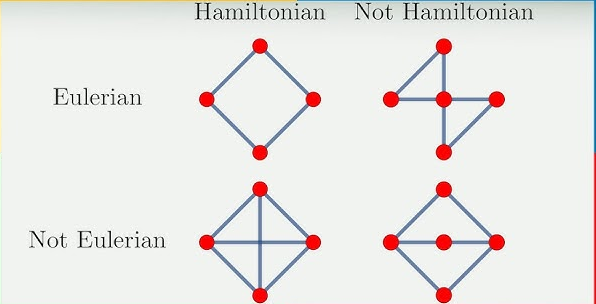
\includegraphics[width=0.66\textwidth]{img-t4/img_413_47.png}
\end{figure}

\newpage

\section{Coloración de grafos}

El problema de la coloración de grafos consiste en asignar un color a cada vértice de un grafo de manera que dos vértices adyacentes no compartan el mismo color. El mínimo número de colores necesarios para realizar esta tarea se denomina el \textbf{número cromático} del grafo y se denota por $\chi(G)$.

\subsection{Propiedades fundamentales}
\begin{itemize}
    \item \textbf{Teorema de los cuatro colores:} Todo grafo plano se puede colorear con \textbf{a lo sumo 4 colores}.
    \item Para un grafo simple $G$, se cumple que:
    \begin{equation}
        1 \leq \chi(G) \leq |V|,
    \end{equation}
    donde $|V|$ es el número de vértices del grafo.
    \item Para un grafo completo $K_n$, el número cromático es igual a $n$: \[\chi(K_n) = n.\]
    \item Para cualquier grafo $G$, el número cromático está acotado por:
    \begin{equation}
        \chi(G) \leq 1 + \Delta(G),
    \end{equation}
    donde $\Delta(G)$ es el \textbf{grado máximo} de los vértices del grafo.
\end{itemize}

\subsection{Grafos bipartitos y ciclos}
\begin{itemize}
    \item Un grafo es \textbf{2-colorable} si y solo si es \textbf{bipartito}.
    \item Si $G$ es un ciclo $C_n$, entonces:
    \begin{itemize}
        \item $\chi(C_n) = 2$ si el ciclo tiene longitud par.
        \item $\chi(C_n) = 3$ si el ciclo tiene longitud impar.
    \end{itemize}
\end{itemize}

\subsection{Teorema de Brooks}
\textbf{Teorema de Brooks:} Sea $G$ un grafo conexo. Si $G$ no es un grafo completo y no contiene ciclos de longitud impar, entonces:
\begin{equation}
    \chi(G) \leq \Delta(G).
\end{equation}

\subsection{Algoritmo voraz para colorear un grafo}
Un método sencillo para colorear un grafo es el \textbf{algoritmo voraz}, que sigue estos pasos:
\begin{enumerate}
    \item Numerar los vértices del grafo.
    \item Colorear el primer vértice con el primer color.
    \item Colorear el segundo vértice con el primer color disponible que no sea usado por sus vecinos.
    \item Repetir este proceso para los siguientes vértices, coloreando cada uno con el primer color disponible.
\end{enumerate}
\textbf{Nota:} Este algoritmo puede no encontrar la coloración óptima, pero asegura que se usen a lo sumo $|V|$ colores, donde $|V|$ es el número de vértices del grafo.

\newpage

\section{Grafo ponderado}

Un grafo $G = (V, E)$ se denomina \textbf{ponderado} si existe una función de peso definida como:
\begin{equation}
    w: E \to \mathbb{R}^+ \cup \{0\}, \quad e \mapsto w(e),
\end{equation}
donde $w(e)$ representa el peso del eje $e$.

\subsection{Propiedades de los árboles en grafos}
Sea $G = (V, E)$ un grafo, se cumplen las siguientes propiedades equivalentes:
\begin{itemize}
    \item $G$ es un \textbf{árbol} \(\iff\) cada par de vértices distintos está conectado por un único camino.
    \item $G$ es \textbf{conexo} y cada eje es un \textbf{eje de separación} (o puente).
    \item $G$ es \textbf{conexo} y $|V| = |E| + 1$.
    \item $G$ no contiene circuitos y $|V| = |E| + 1$.
\end{itemize}

\subsection{Árboles generadores}
Sea $G$ un grafo conexo. Un \textbf{árbol generador} (también llamado \textit{recubridor} o \textit{spanning tree}) es un subgrafo $T$ de $G$ que:
\begin{itemize}
    \item Es un árbol.
    \item Conecta todos los vértices del grafo.
\end{itemize}

Un árbol generador se dice \textbf{minimal} si su peso es el mínimo posible entre todos los árboles generadores de $G$.

\subsection{Algoritmo de Kruskal}
El algoritmo de \textbf{Kruskal} es un método voraz para encontrar un árbol generador minimal. Su procedimiento es el siguiente:
\begin{enumerate}
    \item Inicializar un contador $i = 1$ y seleccionar el eje de peso mínimo $e_1$ del grafo.
    \item Mientras $1 \leq i \leq |V| - 2$:
    \begin{enumerate}
        \item Tomar el eje $e_{i+1}$ de peso mínimo entre los ejes restantes del grafo que no formen un circuito con los ejes $e_1, e_2, \dots, e_i$.
        \item Incrementar $i$.
    \end{enumerate}
    \item Repetir el paso anterior hasta que no se puedan seleccionar más ejes.
\end{enumerate}

\subsection{Algoritmo de Prim}
El algoritmo de \textbf{Prim} es otro método voraz para encontrar un árbol generador minimal. Su procedimiento es el siguiente:
\begin{enumerate}
    \item Seleccionar un vértice cualquiera $v$ como punto de inicio. Inicializar $T_0 = \{v\}$ (primer árbol).
    \item Considerar el conjunto de ejes que inciden en alguno de los vértices del árbol $T_i$ construido hasta el momento. Seleccionar el eje de peso mínimo que no forme un circuito con los ejes del árbol y añadirlo al árbol.
    \item Repetir el paso anterior hasta que no se puedan añadir más ejes.
\end{enumerate}

\section{El Algoritmo de Hierholzer}

El algoritmo de Hierholzer es un método eficiente para \textbf{encontrar un ciclo Euleriano en un grafo conexo donde todos los vértices tienen un grado par}. Se aplica principalmente en \textbf{grafos no dirigidos}, aunque también puede adaptarse para grafos dirigidos.

\subsection{Descripción del Algoritmo}

El algoritmo de Hierholzer sigue estos pasos:

\begin{enumerate}
    \item Selecciona un vértice inicial arbitrario del grafo.
    \item Construye un ciclo inicial siguiendo aristas no utilizadas hasta regresar al vértice de inicio.
    \item Si aún quedan aristas no utilizadas, selecciona un vértice en el ciclo actual que tenga aristas no utilizadas y construye un subciclo desde este vértice.
    \item Fusiona el subciclo con el ciclo original.
    \item Repite los pasos 3 y 4 hasta que todas las aristas hayan sido utilizadas.
\end{enumerate}

\subsection{Ejemplo}

Consideremos el siguiente grafo no dirigido con los vértices y aristas:

\begin{itemize}
    \item Vértices: \( \{A, B, C, D\} \)
    \item Aristas: \( \{(A, B), (A, C), (B, C), (B, D), (C, D)\} \)
\end{itemize}

El grafo es conexo y todos los vértices tienen un grado par, por lo que cumple las condiciones para tener un ciclo Euleriano. Aplicamos el algoritmo:

\begin{enumerate}
    \item Seleccionamos \( A \) como vértice inicial.
    \item Construimos un ciclo inicial: \( A \to B \to C \to A \).
    \item El vértice \( B \) tiene una arista no utilizada (\( B \to D \)). Construimos un subciclo desde \( B \): \( B \to D \to C \to B \).
    \item Fusionamos el subciclo con el ciclo original: \( A \to B \to D \to C \to B \to C \to A \).
\end{enumerate}

Por lo tanto, el ciclo Euleriano encontrado es \( A \to B \to D \to C \to B \to C \to A \).

\subsection{Complejidad}

El algoritmo de Hierholzer tiene una complejidad temporal de \( O(E) \), donde \( E \) es el número de aristas del grafo. Esto se debe a que cada arista se recorre exactamente una vez.



\begin{comment}
\begin{figure}[h]
    \centering
    \includegraphics[width=0.5\textwidth]{1.png}
    \caption{}
\end{figure}
\end{comment}

\begin{comment}
\begin{wrapfigure}[]{r}{0.5\linewidth}
    \centering
    \includegraphics[width=\linewidth]{8.png}
    \caption{}
\end{wrapfigure}
\end{comment}

\end{document}